\documentclass[tikz,border=2pt]{standalone}
\usepackage{lmodern}
\usepackage{amsmath,amssymb,bm}
\usetikzlibrary{decorations.pathmorphing}
\definecolor{ink}{HTML}{1B2B37}
\definecolor{blue}{HTML}{087CAB}
\definecolor{orange}{HTML}{CE641B}
\definecolor{muted}{HTML}{596B77}
\tikzset{
  paired/.style={font=\fontsize{10}{12}\selectfont,text=ink,
    align=center,inner sep=1pt},
  mediator/.style={font=\sffamily\fontsize{9}{11}\selectfont,
    text=ink,align=center,inner sep=1pt},
  leg/.style={line width=.85pt,decorate,
    decoration={snake,amplitude=.55mm,segment length=3.1mm,
      pre length=1mm,post length=1.3mm}},
  internal/.style={line width=1.1pt,decorate,
    decoration={snake,amplitude=.65mm,segment length=3.3mm,
      pre length=1.2mm,post length=1.5mm}},
}
\begin{document}
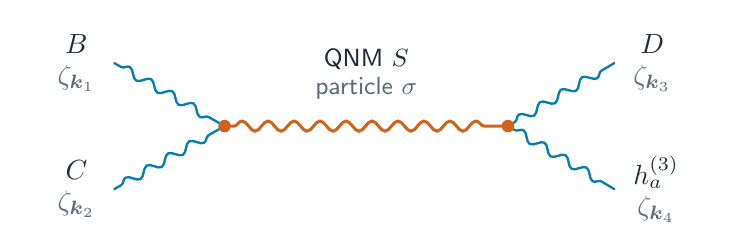
\begin{tikzpicture}[x=1cm,y=1cm,line cap=round,line join=round]
\useasboundingbox (0,.08) rectangle (8.6,2.55);
\coordinate (leftVertex) at (2.50,1.30);
\coordinate (rightVertex) at (6.10,1.30);
\draw[leg,blue] (1.10,2.10)--(leftVertex);
\draw[leg,blue] (1.10,.50)--(leftVertex);
\draw[internal,orange] (leftVertex)--(rightVertex);
\draw[leg,blue] (rightVertex)--(7.45,2.10);
\draw[leg,blue] (rightVertex)--(7.45,.50);
\fill[orange] (leftVertex) circle (.080);
\fill[orange] (rightVertex) circle (.080);
\node[paired,anchor=east] at (.90,2.10)
  {$B$\\[-1pt]\textcolor{muted}{$\zeta_{\bm k_1}$}};
\node[paired,anchor=east] at (.90,.50)
  {$C$\\[-1pt]\textcolor{muted}{$\zeta_{\bm k_2}$}};
\node[paired,anchor=west] at (7.65,2.10)
  {$D$\\[-1pt]\textcolor{muted}{$\zeta_{\bm k_3}$}};
\node[paired,anchor=west] at (7.65,.50)
  {$h_a^{(3)}$\\[-1pt]\textcolor{muted}{$\zeta_{\bm k_4}$}};
\node[mediator,anchor=south] at (4.30,1.60)
  {QNM $S$\\[-1pt]\textcolor{muted}{particle $\sigma$}};
\end{tikzpicture}
\end{document}
